\documentclass[12pt,a4paper]{article}

% ─── Page Layout ───────────────────────────────────────────────────────────────
\usepackage[a4paper, margin=0.8in, headheight=14pt]{geometry}

% ─── Fonts (XeLaTeX) ───────────────────────────────────────────────────────────
\usepackage{fontspec}
\usepackage{unicode-math}
\setmainfont{TeX Gyre Pagella}
\setmonofont[Scale=0.88]{TeX Gyre Cursor}
\setmathfont{Latin Modern Math}

% ─── Packages ──────────────────────────────────────────────────────────────────
\usepackage{xcolor}
\usepackage{colortbl}
\usepackage{titlesec}
\usepackage{enumitem}
\usepackage{tabularx}
\usepackage{booktabs}
\usepackage{array}
\usepackage{amsmath}
\usepackage{tikz}
\usetikzlibrary{shapes.geometric, arrows.meta, positioning, calc, fit, decorations.pathreplacing, patterns}
\usepackage{tcolorbox}
\tcbuselibrary{skins, breakable}
\usepackage{hyperref}
\usepackage{fancyhdr}
\usepackage{graphicx}
\usepackage{microtype}
\hyphenpenalty=10000
\exhyphenpenalty=10000
\sloppy
\usepackage{caption}
\usepackage{setspace}
\usepackage{multirow}
\usepackage{tocloft}

% ─── Q&A helper ────────────────────────────────────────────────────────────────
\newcommand{\Q}[1]{\textbf{#1}\par\noindent\ignorespaces}

% ─── Colour Palette ────────────────────────────────────────────────────────────
\definecolor{myred}{RGB}{196,30,58}
\definecolor{mydark}{RGB}{30,30,50}
\definecolor{mygreen}{RGB}{14,120,80}
\definecolor{myteal}{RGB}{0,130,140}
\definecolor{myamber}{RGB}{180,100,0}
\definecolor{mypurple}{RGB}{100,30,160}
\definecolor{mygray}{RGB}{246,247,249}
\definecolor{mgframe}{RGB}{180,185,200}
\definecolor{watermark}{RGB}{145,150,170}
\definecolor{hdrred}{RGB}{250,232,235}
\definecolor{hdrgreen}{RGB}{220,244,233}
\definecolor{hdrteal}{RGB}{220,242,244}
\definecolor{hdramber}{RGB}{253,242,215}
\definecolor{hdrpurple}{RGB}{238,228,255}
\definecolor{hdrgray}{RGB}{238,240,245}
\definecolor{rowalt}{RGB}{250,251,253}

% ─── Section Formatting ────────────────────────────────────────────────────────
\titleformat{\section}
  {\large\bfseries\color{myred}}{\thesection.}{0.5em}{}
  [\vspace{1pt}{\color{myred}\rule{\linewidth}{0.8pt}}]
\titleformat{\subsection}
  {\normalsize\bfseries\color{myteal}}{\thesubsection}{0.5em}{}
\titlespacing*{\section}{0pt}{18pt}{7pt}
\titlespacing*{\subsection}{0pt}{11pt}{4pt}

% ─── Paragraph ─────────────────────────────────────────────────────────────────
\setlength{\parindent}{0pt}
\setlength{\parskip}{4pt}

% ─── TOC Styling ───────────────────────────────────────────────────────────────
\renewcommand{\cfttoctitlefont}{\large\bfseries\color{myred}}
\renewcommand{\cftaftertoctitle}{\par\noindent{\color{myred}\rule{\linewidth}{0.8pt}}}
\setlength{\cftbeforetoctitleskip}{0pt}
\setlength{\cftaftertoctitleskip}{6pt}
\renewcommand{\cftsecfont}{\normalsize\bfseries\color{mydark}}
\renewcommand{\cftsecpagefont}{\normalsize\bfseries\color{mydark}}
\renewcommand{\cftsecleader}{\cftdotfill{\cftdotsep}}
\setlength{\cftbeforesecskip}{7pt}
\renewcommand{\cftsubsecfont}{\small\color{mydark}}
\renewcommand{\cftsubsecpagefont}{\small\color{mydark}}
\setlength{\cftbeforesubsecskip}{3pt}
\setlength{\cftsubsecindent}{1.4em}

% ─── Table helpers ─────────────────────────────────────────────────────────────
\renewcommand{\arraystretch}{1.45}
\setlength{\tabcolsep}{6pt}
\arrayrulecolor{mydark}
\newcolumntype{B}[1]{>{\small\bfseries\raggedright\arraybackslash}m{#1}}
\newcolumntype{Y}{>{\small\raggedright\arraybackslash}X}
\renewcommand{\tabularxcolumn}[1]{m{#1}}

% ─── Header / Footer ───────────────────────────────────────────────────────────
\pagestyle{fancy}
\fancyhf{}
\fancyhead[L]{\small\color{myred}\textbf{26-ES-EE101}\;\color{mydark}--- Basic Electrical and Electronics Engineering}
\fancyhead[R]{\small\color{myteal}\textbf{Module 1 Notes}}
\fancyfoot[C]{\small\color{mydark}\thepage}
\fancyfoot[R]{\small\color{watermark}\textit{\copyright\ Biraj}}
\renewcommand{\headrulewidth}{0.5pt}
\renewcommand{\footrulewidth}{0.3pt}

% ─── Hyperref ──────────────────────────────────────────────────────────────────
\hypersetup{
  colorlinks=true, linkcolor=myteal, urlcolor=myteal,
  pdfauthor={Biraj Sarkar (CGEC)},
  pdftitle={26-ES-EE101 --- Module 1 Notes: Basics of Electrical Wiring and Safety}
}

% ─── tcolorbox styles ──────────────────────────────────────────────────────────
\tcbset{
  tikzbox/.style={
    colback=mygray, colframe=mgframe, boxrule=0.6pt, arc=4pt,
    left=8pt, right=8pt, top=6pt, bottom=6pt,
    colbacktitle=mgframe, coltitle=mydark, fonttitle=\small\bfseries
  },
  defbox/.style={
    colback=hdrgreen, colframe=mygreen, boxrule=0.8pt, arc=4pt,
    left=9pt, right=9pt, top=6pt, bottom=6pt,
    colbacktitle=mygreen, coltitle=white, fonttitle=\small\bfseries
  },
  formulabox/.style={
    colback=hdrteal, colframe=myteal, boxrule=0.8pt, arc=4pt,
    left=9pt, right=9pt, top=7pt, bottom=7pt,
    colbacktitle=myteal, coltitle=white, fonttitle=\small\bfseries
  },
  examplebox/.style={
    colback=hdramber, colframe=myamber, boxrule=0.8pt, arc=4pt,
    left=9pt, right=9pt, top=6pt, bottom=6pt,
    colbacktitle=myamber, coltitle=white, fonttitle=\small\bfseries
  },
  masonbox/.style={
    colback=hdrpurple, colframe=mypurple, boxrule=0.8pt, arc=4pt,
    left=9pt, right=9pt, top=6pt, bottom=6pt,
    colbacktitle=mypurple, coltitle=white, fonttitle=\small\bfseries
  },
  exambox/.style={
    colback=hdrpurple, colframe=mypurple, boxrule=1pt, arc=5pt,
    left=10pt, right=10pt, top=8pt, bottom=8pt,
    colbacktitle=mypurple, coltitle=white, fonttitle=\bfseries,
    breakable, title after break={\textbf{Frequently Asked / Viva Questions (contd.)}}
  }
}
\tcbset{breakable}
\tcbset{after={\par\color{black}}}

% ─── TikZ styles ───────────────────────────────────────────────────────────────
\tikzset{
  block/.style={rectangle, draw=myteal, fill=hdrteal,
    text width=2.4cm, align=center, minimum height=0.95cm,
    font=\small, rounded corners=3pt, line width=0.7pt},
  redblock/.style={rectangle, draw=myred, fill=hdrred,
    text width=2.4cm, align=center, minimum height=0.95cm,
    font=\small, rounded corners=3pt, line width=0.7pt},
  sumjunc/.style={circle, draw=myamber, fill=hdramber,
    minimum size=0.62cm, font=\small, line width=0.8pt},
  arrow/.style={-Stealth, thick, color=mydark},
  redarrow/.style={-Stealth, thick, color=myred},
  line/.style={thick, color=mydark}
}

\begin{document}

% ─── Title Page ───────────────────────────────────────────────────────────────
\begin{center}
  {\Large\bfseries\color{myred} 26-ES-EE101}\\[3pt]
  {\LARGE\bfseries\color{myred} Basic Electrical and Electronics Engineering}\\[5pt]
  {\normalsize\color{mydark} Semester I \quad$\bullet$\quad 3L:1T:0P \quad$\bullet$\quad 4 Credits}\\[3pt]
  {\normalsize\color{myteal}\textbf{Module 1 Exam Notes: Basics of Electrical Wiring and Safety}}\\[3pt]
  {\small\color{mydark} CGEC \;$|$\; MAKAUT Syllabus (A.Y. 2026--27) \;$|$\; \textit{Biraj Sarkar}}
\end{center}
\vspace{2pt}
\noindent{\color{myred}\rule{\linewidth}{1.5pt}}
\vspace{2pt}

\hypersetup{linkcolor=mydark}
\tableofcontents
\hypersetup{linkcolor=myteal}
\newpage

\section{Basics of Electrical Wiring and Safety}

\subsection{Electric shock and earthing}

\begin{tcolorbox}[defbox,title={Electric shock and protective earthing}]
Electric shock is the harmful effect of current passing through the body. Protective earthing connects exposed conductive parts, such as a metal appliance enclosure, to the protective earth system.
\end{tcolorbox}

\begin{itemize}[leftmargin=*, itemsep=3pt, topsep=4pt]
  \item \textbf{Effects.} Current through tissue can cause pain, muscle contraction, breathing difficulty, ventricular fibrillation and burns.
  \item \textbf{Severity.} It depends on current, duration, frequency, path and skin condition. A chest-crossing path is especially dangerous. Wet skin usually has a lower resistance.
  \item \textbf{Current estimate.} \(I=V/Z_{\mathrm{body}}\) explains the trend. Body impedance varies, so the estimate alone cannot establish a safe touch voltage.
\end{itemize}

\begin{itemize}[leftmargin=*, itemsep=3pt, topsep=4pt]
  \item \textbf{Normal condition.} Neutral carries the load return current. The protective-earth conductor carries negligible load current and serves a separate function downstream of the supply arrangement.
  \item \textbf{Fault on the case.} The earth bond gives fault current a return path, helps limit touch voltage and supports automatic disconnection.
  \item \textbf{Disconnection.} A fuse or breaker responds if the fault loop current is sufficient. A residual-current device (RCD) can respond to a much smaller leakage current.
\end{itemize}

\begin{tcolorbox}[tikzbox,title={Protective roles in a single-phase circuit},unbreakable]
\centering
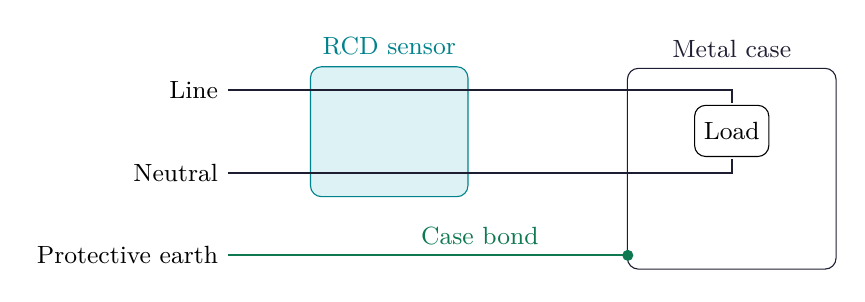
\begin{tikzpicture}[font=\small]
\node[left] at (0,2.2) {Line};
\node[left] at (0,1.15) {Neutral};
\node[left] at (0,0.1) {Protective earth};
\node[draw=myteal,fill=hdrteal,minimum width=2.0cm,minimum height=1.65cm,rounded corners] at (2.05,1.67) {};
\node[myteal,above] at (2.05,2.52) {RCD sensor};
\node[draw=mydark,minimum width=2.65cm,minimum height=2.55cm,rounded corners] (case) at (6.4,1.2) {};
\node[mydark,above] at (6.4,2.48) {Metal case};
\draw[line] (0,2.2)--(6.4,2.2)--(6.4,2.04);
\draw[line] (0,1.15)--(6.4,1.15)--(6.4,1.32);
\node[draw,rounded corners,fill=white,minimum height=0.65cm] at (6.4,1.68) {Load};
\draw[mygreen,thick] (0,0.1)--(5.08,0.1) node[pos=0.63,above] {Case bond};
\fill[mygreen] (5.08,0.1) circle (2pt);
\end{tikzpicture}
\end{tcolorbox}

For a shock incident, disconnect the supply safely before approaching the person, avoid direct contact while the supply may be live, and call emergency help. Repairs and inspection require isolation and verification by a competent person. In a written answer, state why earthing and automatic disconnection work together.

\subsection{Protective and switching devices}

\begin{itemize}[leftmargin=*, itemsep=3pt, topsep=4pt]
  \item \textbf{Overload.} Excessive current in a healthy circuit, often from too much connected load.
  \item \textbf{Short circuit.} Unintended low-impedance connection between points at different potentials.
  \item \textbf{Earth fault.} Unintended current from a live part to earth or to an earthed part.
\end{itemize}

An \textbf{RCD} detects the imbalance between currents in the live conductors passing through its sensor. In a healthy single-phase circuit the line and neutral currents cancel in the sensor. A leakage return outside the sensor gives a residual current:
\[
I_{\Delta}=\lvert I_L-I_N\rvert .
\]
An RCCB provides residual-current protection. An RCBO combines residual-current and overcurrent protection. A person touching line and neutral simultaneously may draw equal currents through both sensed conductors, so a residual-current device alone cannot be relied on in that case.

\par\vspace{6pt}\noindent
\begin{tabularx}{\linewidth}{|B{3.0cm}|Y|Y|}\hline
Device & \textbf{Working principle} & \textbf{Typical role} \\ \hline
SFU (switch-fuse unit) & A rated manual switch and fuse links. A link melts on excess current and is replaced after the fault is corrected. & Feeder isolation and overcurrent protection. \\ \hline
MCB (miniature circuit breaker) & Thermal action for overload and magnetic action for severe fault current in a typical thermal-magnetic design. Can be reset after clearing the fault. & Final-circuit overcurrent protection. \\ \hline
ELCB (earth leakage circuit breaker) & A traditional voltage-operated ELCB senses voltage rise on the protected earth system. The term is also used loosely for current-operated residual-current devices. & Earth-leakage protection. Identify the sensing principle explicitly in an answer. \\ \hline
MCCB (moulded-case circuit breaker) & A breaker for higher current or breaking-capacity duties, with thermal-magnetic or electronic trip depending on the design. & Distribution and industrial feeders. Some models offer adjustable settings. \\ \hline
\end{tabularx}

\begin{tcolorbox}[examplebox,title={Reading an RCD example}]
Suppose the line carries \(5.00\,\mathrm A\), and \(4.96\,\mathrm A\) returns through the sensed neutral.
\[
\begin{aligned}
I_\Delta &= \lvert 5.00-4.96\rvert\,\mathrm A\\
         &= 0.04\,\mathrm A\\
         &= 40\,\mathrm{mA}.
\end{aligned}
\]
This exceeds the \(30\,\mathrm{mA}\) rating of the device in this example. Actual disconnection depends on the RCD type and its operating conditions. The \(30\,\mathrm{mA}\) value is a device rating.
\end{tcolorbox}

\subsection{Wires, cables and Indian wiring practice}

A wire is an individual conductor, usually insulated where used in an installation. A cable is an assembly of one or more insulated conductors with any required sheath, screening or armour. Conductor cross-sectional area is expressed in \(\mathrm{mm^2}\). Copper and aluminium are common conductors. Stranding improves flexibility. PVC and XLPE are examples of insulation. A sheath protects against the environment, while armour provides mechanical protection when the service conditions require it.

Typical examples include solid or stranded single-core wires in conduit, multicore sheathed cables for fixed runs, flexible cords for movable appliances, and armoured cables for harsher routes. Selection depends on current capacity, permissible voltage drop, short-circuit withstand, mechanical duty, ambient temperature and grouping. The cable rating and the protection rating must be coordinated.

\begin{itemize}[leftmargin=*, itemsep=3pt, topsep=4pt]
  \item \textbf{Supply path.} Service connection, energy meter, main isolation, then distribution board and individual lighting and power circuits.
  \item \textbf{Distribution board.} Houses circuit protection and uses separate neutral and protective-earth connections as required by the earthing system.
  \item \textbf{Switch and outlet.} A switch or single-pole fuse in the line conductor interrupts the live feed. A three-pin outlet provides line, neutral and protective earth.
  \item \textbf{Wiring methods.} Conduit supports and protects conductors. Casing-and-capping and batten wiring are older methods.
\end{itemize}

Label line, neutral and protective earth as \(\mathrm{L}\), \(\mathrm{N}\) and \(\mathrm{PE}\). Common modern colours are brown, blue and green/yellow respectively. Verify each conductor's function because colours vary with age and standard. Before service, check earthing, polarity, continuity, insulation and protection.

\subsection{Batteries and their characteristics}

\begin{tcolorbox}[defbox,title={Cell, battery and capacity}]
A cell converts chemical energy to electrical energy. A battery contains one or more cells. Capacity (Ah) is the charge delivered under specified conditions.
\end{tcolorbox}

\begin{itemize}[leftmargin=*, itemsep=3pt, topsep=4pt]
  \item \textbf{Primary cells.} Intended for one discharge life. Alkaline cells are an example.
  \item \textbf{Secondary cells.} Rechargeable types include lead-acid (starting and backup), nickel-metal hydride and high-specific-energy lithium-ion. Use suitable charging and protection.
  \item \textbf{Compare cells by} voltage, capacity, energy, internal resistance, discharge rate, cycle life, self-discharge and charging needs. Capacity varies with load, temperature and cut-off voltage.
\end{itemize}

During discharge, \(V_t=E-Ir\), where \(E\) is open-circuit voltage and \(r\) is internal resistance. Matched cells add voltage in series and Ah in balanced parallel at the same voltage. A \(1C\) discharge current in amperes equals the capacity rating in Ah.

\begin{tcolorbox}[examplebox,title={Series battery rating and energy}]
Four \(3.2\,\mathrm V,\ 2\,\mathrm{Ah}\) cells in series retain \(Q_{\mathrm{pack}}=2\,\mathrm{Ah}\).
\[
\begin{aligned}
V_{\mathrm{pack}} &= 4(3.2)=12.8\,\mathrm V,\\
E_{\mathrm{nom}} &\approx V_{\mathrm{pack}}Q_{\mathrm{pack}}=12.8(2)=25.6\,\mathrm{Wh}.
\end{aligned}
\]
Ah measures charge. Wh measures energy (\(1\,\mathrm{Wh}=3600\,\mathrm J\)).
\end{tcolorbox}

\newpage
\begin{center}
  {\large\bfseries\color{myred} Quick Revision --- Module 1}\\[3pt]
  {\small\color{mydark} Basics of Electrical Wiring and Safety $|$ 26-ES-EE101}
\end{center}
\noindent{\color{myred}\rule{\linewidth}{1.2pt}}
\vspace{4pt}

\begin{tcolorbox}[formulabox, title={Key Formulas and Concepts at a Glance}]
\renewcommand{\arraystretch}{1.35}
\begin{tabularx}{\linewidth}{B{4.4cm}Y}
Residual current & $I_\Delta=\lvert I_L-I_N\rvert$ in A. \\[3pt]
Battery terminal voltage & $V_t=E-Ir$ during discharge. \\[3pt]
Nominal battery energy & $E_{\mathrm{nom}}\approx V_{\mathrm{nom}}Q$ in Wh for $Q$ in Ah. \\[3pt]
\end{tabularx}
\end{tcolorbox}

\begin{tcolorbox}[defbox, title={One-Line Definitions}]
\textbf{Protective earthing.} Bonding exposed conductive parts to the protective earth system.

\textbf{Breaking capacity.} Prospective fault current that a device can safely interrupt under its rated conditions.

\textbf{Self-discharge.} Loss of stored charge while a battery is idle.
\end{tcolorbox}

\begin{tcolorbox}[exambox, title={Frequently Asked / Viva Questions}]
\begin{enumerate}[topsep=0pt, label=\textbf{Q\arabic*.}, itemsep=5pt]
  \item \Q{What affects shock severity?} Current, duration, path, frequency and body conditions.
  \item \Q{Why earth a metal case?} The bond provides a fault path and supports fast disconnection.
  \item \Q{What does an RCD sense?} The nonzero sum of the currents in the monitored live conductors.
  \item \Q{Can an RCCB replace an MCB?} An RCCB covers residual current. The circuit also needs suitable overcurrent protection.
  \item \Q{How does an MCB distinguish overload and short circuit?} In the usual design a thermal element acts on sustained overload and a magnetic element acts rapidly on large fault current.
  \item \Q{What does SFU stand for?} Switch-fuse unit.
  \item \Q{What does armour do?} It gives mechanical protection to the cable.
  \item \Q{What is the role of a distribution board?} It divides the supply into final circuits and houses their protection.
  \item \Q{Which battery types can be recharged?} Secondary cells and batteries designed for repeated charge and discharge.
  \item \Q{What changes when matched cells are connected in series?} Voltages add and the ampere-hour capacity stays equal to that of one cell.
\end{enumerate}
\end{tcolorbox}

\begin{tcolorbox}[tikzbox, title={Summary Reference}]
\begin{tabularx}{\linewidth}{|B{4.0cm}|Y|}\hline
Topic & \textbf{What to remember} \\ \hline
Protection & Coordinate earthing, residual-current detection and overcurrent protection. \\ \hline
Wiring & Identify line, neutral and protective earth and state their separate functions. \\ \hline
Battery & State voltage and Ah separately and use Wh for energy. \\ \hline
\end{tabularx}
\end{tcolorbox}

\end{document}

